\documentclass[../../main.tex]{subfiles}
\begin{document}

\begin{flushright}
  \footnotesize\textit{【自動文字起こし・要確認】}
\end{flushright}

[解] (1) $\angle \mathrm{APQ} = \theta$とおく．$\theta = 0$の時，$s=3$, $t=2 \cdots \text{\textcircled{1}}$

である．

\begin{figure}[H]
  \centering
  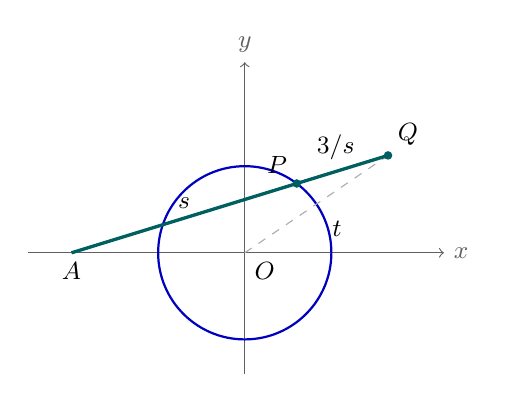
\begin{tikzpicture}[scale=1.1,every node/.style={font=\small}]
    % P=(3/5,4/5) とした配置例．Q は AP・PQ=3 から定まる．
    \coordinate (O) at (0,0);
    \coordinate (A) at (-2,0);
    \coordinate (P) at (0.6,0.8);
    \coordinate (Q) at (1.654,1.124);
    \draw[->,gray!75!black] (-2.5,0)--(2.3,0) node[right] {$x$};
    \draw[->,gray!75!black] (0,-1.4)--(0,2.2) node[above] {$y$};
    \draw[blue!75!black,thick] (O) circle (1);
    \draw[gray!65,dashed] (O)--(Q);
    \draw[teal!75!black,very thick] (A)--(Q);
    \fill[teal!75!black] (P) circle (1.4pt) (Q) circle (1.4pt);
    \node[below right] at (O) {$O$};
    \node[below] at (A) {$A$};
    \node[above left] at (P) {$P$};
    \node[above right] at (Q) {$Q$};
    \node[above] at (-0.7,0.4) {$s$};
    \node[above] at (1.05,0.96) {$3/s$};
    \node[below right] at (0.9,0.48) {$t$};
  \end{tikzpicture}
  \caption{線分$AP$を延長して点$Q$をとる}
\end{figure}

$\theta \neq 0$の時，$\triangle \mathrm{OAP}, \triangle \mathrm{OAQ}$に余弦定理を用いて，
$$
\begin{cases}
  1 = 2^2 + s^2 - 2 \cdot 2 \cdot s \cos\theta \\
  t^2 = 2^2 + \left(s + \dfrac{3}{5}\right)^2 - 2 \cdot 2 \cdot \left(s + \dfrac{3}{5}\right) \cos\theta
\end{cases}
$$
第1式から，$\cos\theta = \dfrac{3+s^2}{4s}$ ($\because s \neq 0$) だから，第2式に代入して，
$$
t^2 = 4 + \left(s + \dfrac{3}{5}\right)^2 - 4 \left(s + \dfrac{3}{5}\right) \dfrac{3+s^2}{4s}
$$
$$
= 4 + \left(s + \dfrac{3}{5}\right)^2 - \left(s + \dfrac{3}{5}\right)^2
$$
$$
= 4
$$
$t > 0$から $t = 2$

\paragraph{(2)}

(1)から，$Q$は$x^2+y^2=4$上にある．さらに，直線$AP$の通過領域内にあれば良いから，

下図の太線の弧（両端を含む）．
\begin{figure}[H]
  \centering
  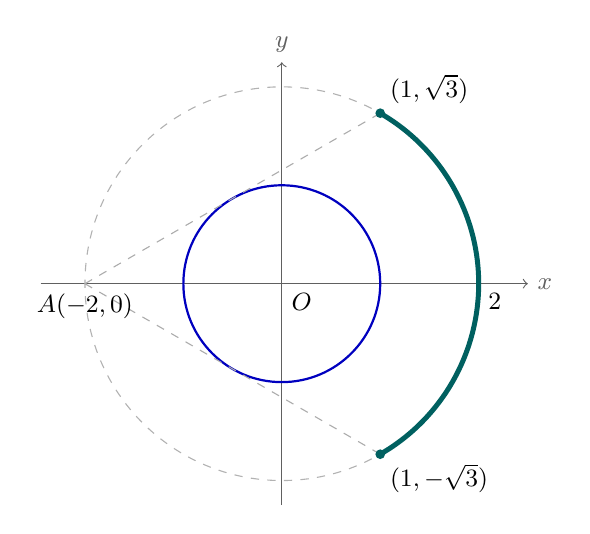
\begin{tikzpicture}[scale=1.25,every node/.style={font=\small}]
    \coordinate (O) at (0,0);
    \coordinate (A) at (-2,0);
    \coordinate (U) at (1,{sqrt(3)});
    \coordinate (L) at (1,{-sqrt(3)});
    \draw[->,gray!75!black] (-2.45,0)--(2.5,0) node[right] {$x$};
    \draw[->,gray!75!black] (0,-2.25)--(0,2.25) node[above] {$y$};
    \draw[gray!60,dashed] (O) circle (2);
    \draw[blue!75!black,thick] (O) circle (1);
    \draw[gray!65,dashed] (A)--(U) (A)--(L);
    \draw[teal!75!black,line width=1.8pt] (L) arc (-60:60:2);
    \fill[teal!75!black] (U) circle (1.4pt) (L) circle (1.4pt);
    \node[below right] at (O) {$O$};
    \node[below] at (A) {$A(-2,0)$};
    \node[above right] at (U) {$(1,\sqrt{3})$};
    \node[below right] at (L) {$(1,-\sqrt{3})$};
    \node[below right] at (2,0) {$2$};
  \end{tikzpicture}
  \caption{点$Q$の軌跡：半径2の円の右側の弧}
\end{figure}

\end{document}
